\clearpage
\subsection{Система с переменной структурой без устойчивого вырожденного движения} \label{title:VSS_no_SDM}
Другой способ построения системы с переменной структурой целесообразно использовать в случае, если фазовое пространство  для каждой из фиксированных структур не содержит гиперплоскостей с устойчивым вырожденным движением. За счёт <<сшивания>> в определенной последовательности участков из неустойчивых траекторий удается получить устойчивое движение для любых начальных условий.

В качестве примера рассмотрим случай, когда в нашем распоряжении имеются две линейные структуры с незатухающими колебаниями, то есть,  находящиеся на границе устойчивости. Уравнения движения в этих системах одно и то же:
\begin{equation} \label{eq:HP_centr}
\cfrac{d^2\,x}{d\,t^2}+\omega_0^2\,x=0
\end{equation}
При разных значениях   фазовые траектории систем  будут иметь вид эллипсов с разными полуосями. Характеристический полином имеет вид:
\begin{equation} \label{eq:HP_centr}
D(p)=p^2+\left(\cfrac{k_{2}}{27}+\cfrac{4}{3}\right)\,p+\cfrac{k_{1}}{27}+\cfrac{1}{81}
\end{equation}
Для получения фазовой траектории типа эллипс необходимо выполнение двух условий:
\begin{equation}
    \left\{
    \begin{aligned} \label{eq:usl_centr1}
       \cfrac{k_{1}}{27}+\cfrac{1}{81}&>0\\
       \cfrac{k_{2}}{27}+\cfrac{4}{3}&=0\\
    \end{aligned}
    \right.
\end{equation}
\begin{equation} \label{eq:}
\Downarrow
\end{equation}
\begin{equation}
    \left\{
    \begin{aligned} \label{eq:usl_centr2}
       k_1&>-0.333\\
       k_2&=-36\\
    \end{aligned}
    \right.
\end{equation}
Пусть $k_1=-0.1667$
Тогда характеристический полином имеет вид:
\begin{equation} \label{eq:elips1}
D(p)=p^2+0.006173
\end{equation}
Пусть $k_1=3.0000$
Тогда характеристический полином имеет вид:
\begin{equation} \label{eq:elips2}
D(p)=p^2+0.1235
\end{equation}
Схема будет иметь тот же вид, что и на рис.\ref{fig:sim_linear_2_por}.
Исследуем движение фазовых координат во времени посредством моделирования процессов в системе при отклонении системы от состояния равновесия. Фазовые траектории в системе на рис.\ref{fig:linear_2_por_ft_center}. 
В дополнение на рис.\ref{fig:linear_2_por_sv_center} указано изменение выходной переменной и её производной. 
\begin{figure}[!h]\centering
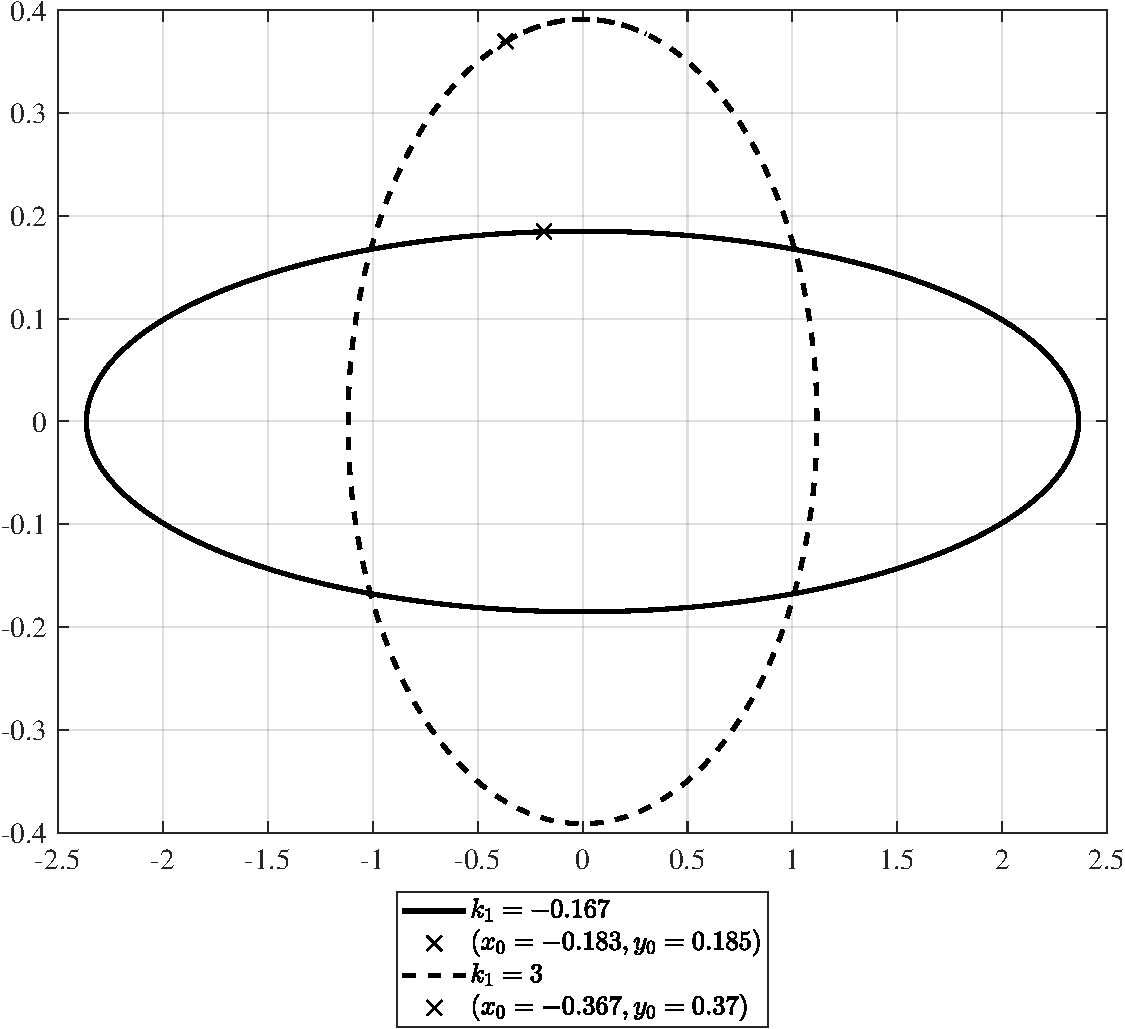
\includegraphics[width=1.0\linewidth]{images/linear_2_por_ft_center}
\caption{ Фазовые траектории для системы с переменной структурой с разными начальными условиями.}\label{fig:linear_2_por_ft_center}
\end{figure}
\begin{figure}[!h]\centering
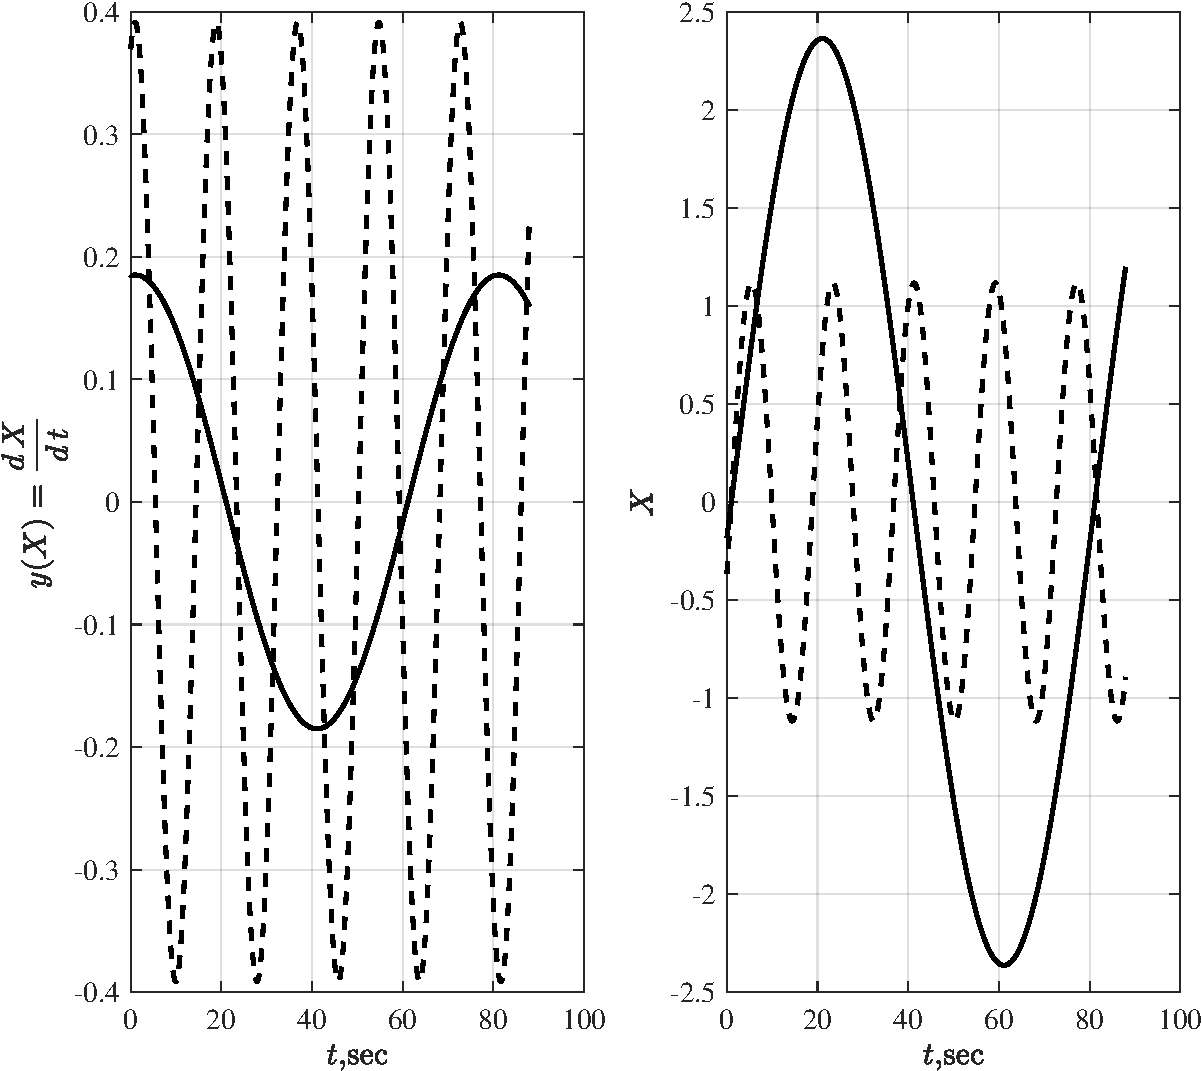
\includegraphics[width=1.0\linewidth]{images/linear_2_por_sv_center}
\caption{ Графики изменения выходной переменной и её производной.}\label{fig:linear_2_por_sv_center}
\end{figure}

Переключение с одной структуры на другую будет происходить при пересечении фазовой траекторией координатных осей. Аналитический закон переключения структур запишется следующим образом:   
\begin{equation}
    \left\{
    \begin{aligned} \label{eq:usl_VSS_center}
       &k_1=3&&,k_2=-36&&,\text{ если }sign(x_1 \cdot x_2)>0\\
       &k_1=-0.167&&,k_2=-36&&,\text{ если }sign(x_1 \cdot x_2)<0\\
    \end{aligned}
    \right.
\end{equation}

Структурная схема системы с переменной структурой без устойчивого вырожденного движения на рис.\ref{fig:sim_VSS_no_steady_degenerate_motion}.
\begin{figure}[!h]\centering
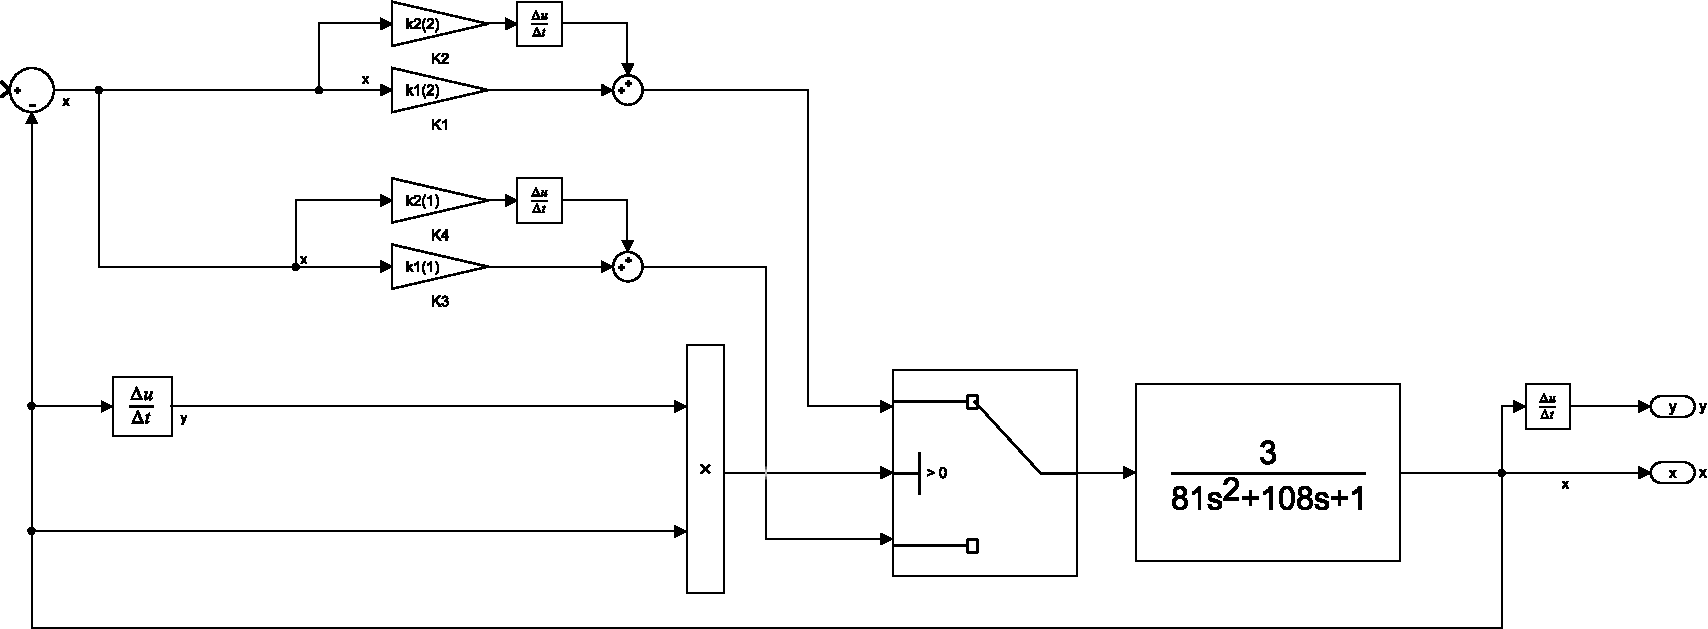
\includegraphics[width=1.0\linewidth]{images/sim_VSS_no_steady_degenerate_motion}
\caption{Структурная схема системы с переменной структурой без устойчивого вырожденного движения}\label{fig:sim_VSS_no_steady_degenerate_motion}
\end{figure}

Исследуем движение фазовых координат во времени посредством моделирования процессов в системе при отклонении системы от состояния равновесия. Фазовые траектории в системе на рис.\ref{fig:VSS_no_steady_degenerate_motion_ft_sedlo}. 
В дополнение на рис.\ref{fig:VSS_no_steady_degenerate_motion_sv_sedlo} указано изменение выходной переменной и её производной. 
\begin{figure}[!h]\centering
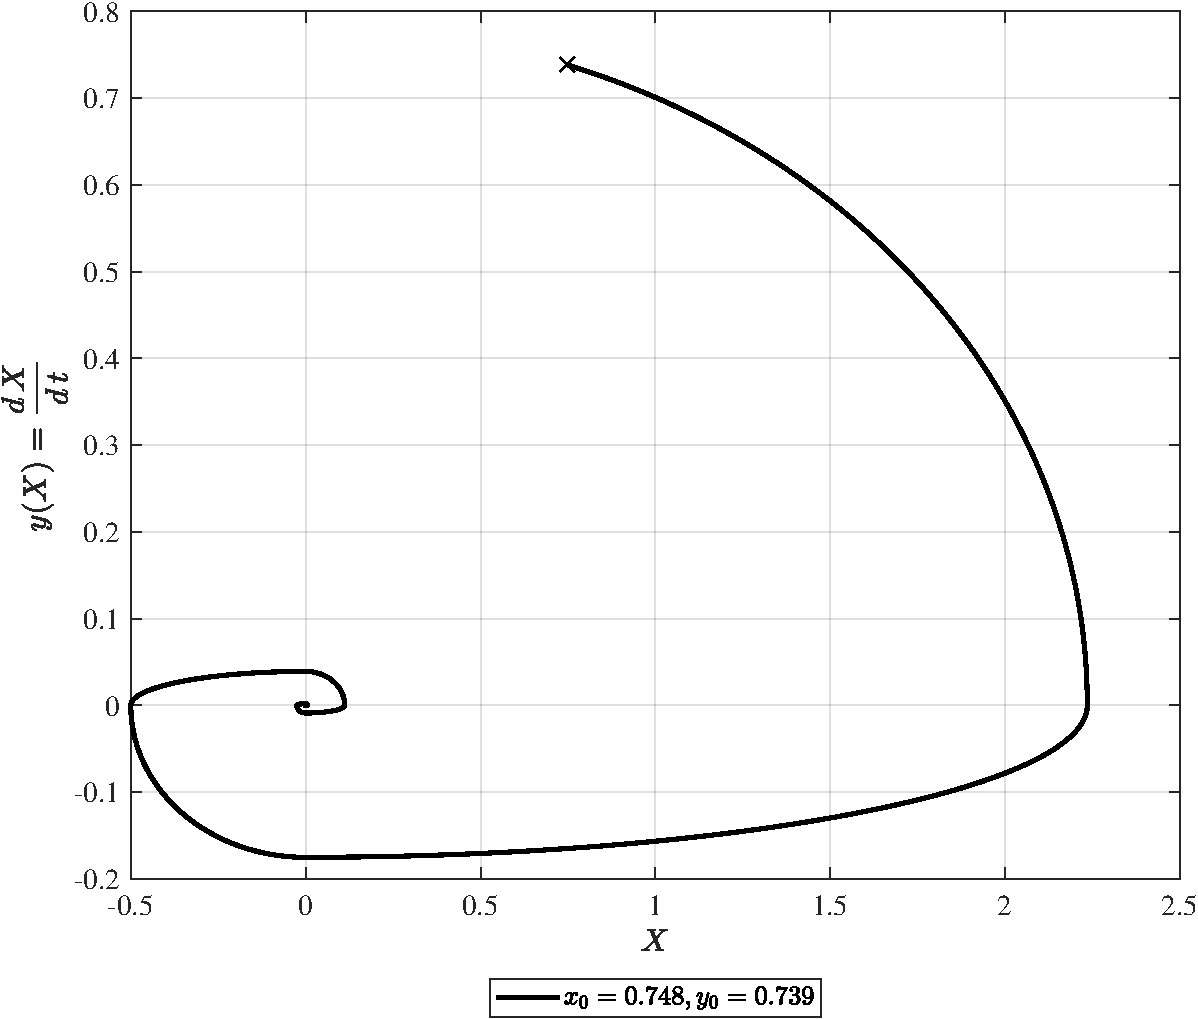
\includegraphics[width=1.0\linewidth]{images/VSS_no_steady_degenerate_motion_ft_sedlo}
\caption{ Фазовые траектории для системы с переменной структурой с разными начальными условиями.}\label{fig:VSS_no_steady_degenerate_motion_ft_sedlo}
\end{figure}
\begin{figure}[!h]\centering
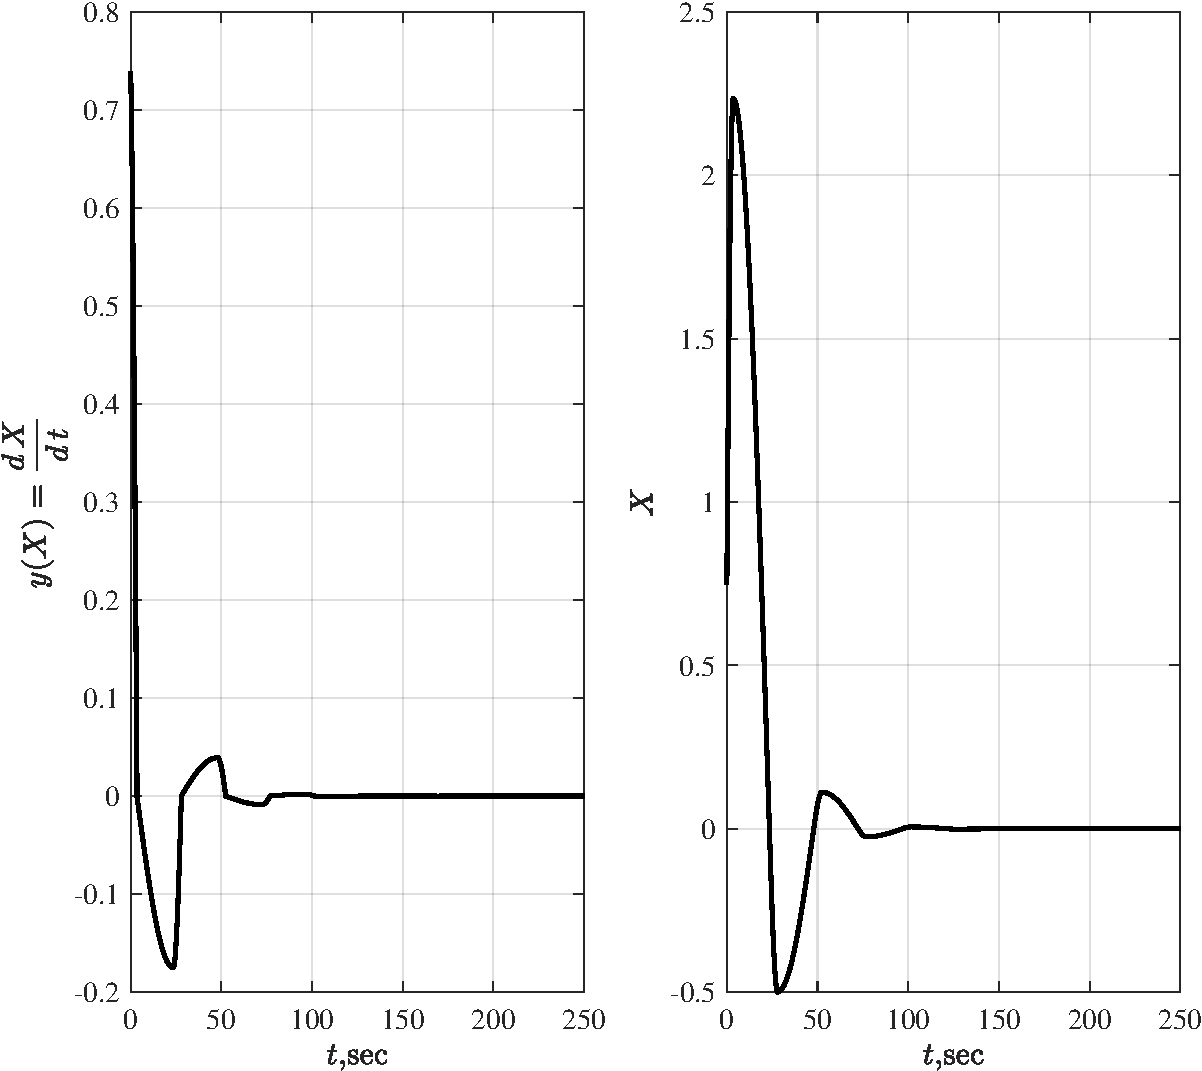
\includegraphics[width=1.0\linewidth]{images/VSS_no_steady_degenerate_motion_sv_sedlo}
\caption{ Графики изменения выходной переменной и её производной.}\label{fig:VSS_no_steady_degenerate_motion_sv_sedlo}
\end{figure}
